% article document class appropriate for small (<100 pages) documents
\documentclass[draft, english, a4paper, 10pt]{article}

% Packages provide additional functionality
%\usepackage{url}
\usepackage{fixme}
%\usepackage{lmodern}
\usepackage[final]{graphicx}%Force the graphics package to final, to force image inclusion
\graphicspath{{eps/}{images/}} %Set images/figures search path (relative to top latex file)
\usepackage[utf8]{inputenc}
\usepackage[left=3cm,top=4cm,right=3cm]{geometry}
\usepackage[dvips,
            colorlinks=false,
            pdfduplex=DuplexFlipLongEdge,
            pdfborder={0 0 0},
            pdftitle={Playing with LEGO},
            pdfauthor={Mikael Moghadam, Kenni Peter Isaksen, Morten S. Laursen,
                Robot Technology,
                SDU,
                Odense,
                Danmark},
            pdfsubject={Introduction to Artificial Intelligence},
            pdfkeywords={LEGO, Sokoban, line follow},
            plainpages=false,
            final]{hyperref}

\title{Playing with LEGO}
\author{Mikael Moghadam, Kenni Peter Isaksen, Morten S. Laursen}

\begin{document}

\maketitle % reads info from \title and \author above


% where BibTeX should read the bibliography records from and what
% style of bibliography it should generate
%\bibliographystyle{plain}
%\bibliography{}
\section{Introduction}
\newpage
\tableofcontents
\newpage
\section{Architecture}
	\subsection{Division of responsibilities}
\section{Robot description}
        The purpose of this prototype is to perform the assignment as described by
        the planner. In order to accomplish this task a robot 
        has been created. The robot is created using the LEGO NXT platform.  
	\subsection{Physical Construction} %Morten  
	    \label{robot:physicalContruction}
	    \fixme{Insert Robot picture here}
	    The robot is constructed using two motors which applies force to
	    each of their front wheels, this allows the robot to steer using skid steering.
	    As close as possible to the center of rotation during turns, three light
	    reflectance sensors is placed as illustrated in figure \ref{fig:lightSensorPlacement}
	    \begin{figure}[htp]
            \centering
    	    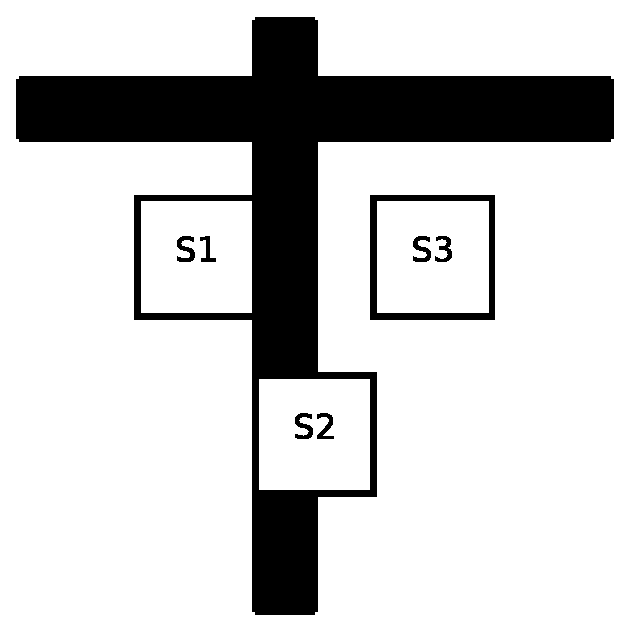
\includegraphics[scale=0.45]{lightSensorPlacement}
	        \caption{Illustration of light sensor placement, with the sensors mentioned S1-S3}\label{fig:lightSensorPlacement}
        \end{figure}
	    This allows the robot to detect either side of the line and thereby to
	    follow it, furthermore it allows the robot to detect when crossing a 
	    line.
	      
	\subsection{Robot architecture}
	    The Software architecture for the robot is devided into layers
	    this is performed to give an abstraction
	    of each layer with as little complexity as possible. The architecture
	    is best illustrated by the block diagram illustrated in figure \ref{fig:robotBlockDiagram}.
	    \begin{figure}[htp]
            \centering
    	    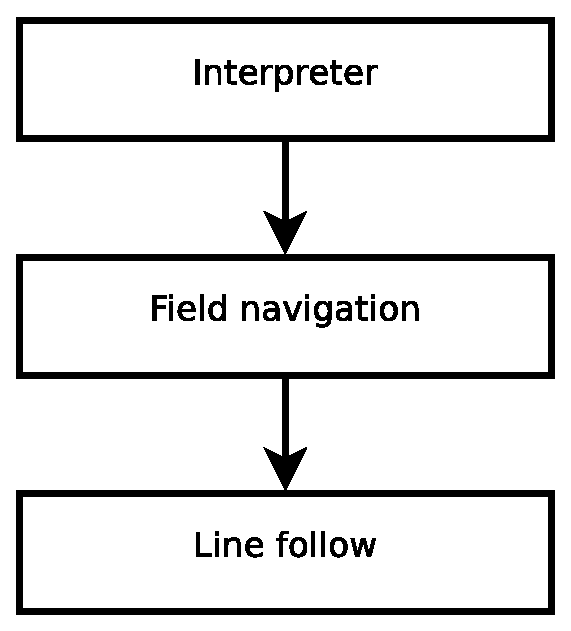
\includegraphics[scale=0.45]{robotBlockdiagram}
	        \caption{Block diagram of LEGO robot}\label{fig:robotBlockDiagram}
        \end{figure}
		%General introduction
		%block diagram
		\subsubsection{Interpreter} %Morten
		    The interpreter has to receive and interpret data from the routeplanner
		    and carry out that route using the field navigation block.\\
		    \\
		    The flow chart for the interpreter can therefore be described in the
		    following way
		    \begin{enumerate}
		    \item Receive/fetch command from routeplanner
		    \item perform command using field navigation
		    \item if more commands in cue goto 1, else exit
		    \end{enumerate}
		    Currently two options is under consideration for the interface between
		    the interpreter and the routeplanner, one is a simple file composed
		    of direction commands as delivered with the Sokoban example game.
		    The other option is to stream the commands using bluetooth, it is
		    anticipated that this would allow for easier debugging, and because
		    of existing libraries for bluetooth it should not cause much if any overhead.\\
		    \\
		    \fixme{For discussion: Should the interpreter or the routeplanner be responsible of
		    tomato can attack directions?}
%			What is the responsibility of this block
%			Block interface
%			Block design / bird perspective flow chart 
%			Block test
		\subsubsection{Field navigation} %Morten
		    The field navigation should navigate between field intersections
		    as illustrated on figure \ref{fig:robotFieldNavigation}.
		    This task should be accomplished using the line following block\\
		    \begin{figure}[htp]
                \centering
    	        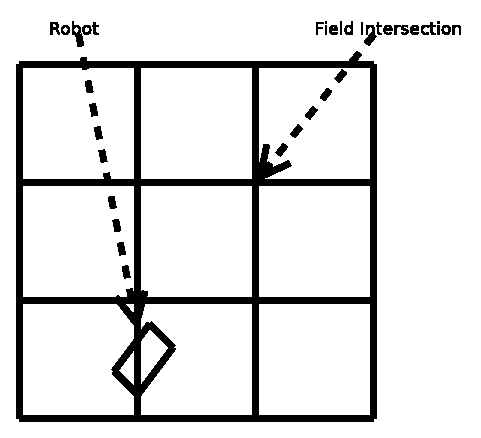
\includegraphics[scale=0.45]{robotFieldNavigation}
	            \caption{Illustration of playing field}\label{fig:robotFieldNavigation}
            \end{figure}
		    \\
		    As described in section \ref{robot:physicalContruction} the light
		    sensors is placed so that when following lines, only one sensor should
		    be active at a time, however when crossing a line both the left and the
		    right sensor should become active. This allows the robot to detect
		    crossing lines.\\
		    \\
		    When crossing a line the robot should first back up, so that the sensors
		    is placed over the crossing line, then rotate in the commanded direction
		    until a new line activates both sensors, then move one field
		    forward.
		    \fixme{Another option here is using the encoders
		    in reality we might test both and see which one performs best}
%			What is the responsibility of this block
%			Block interface
%			Block design / bird perspective flow chart 
%			Block test
		\subsubsection{Line follow} %Morten
		    The line following block has the responsibility of keeping the robot
		    constantly on the line using the sensors to allow for precise navigation.\\
		    \\
		    On figure \ref{fig:sensor_measurements} a plot of what the sensors
		    measures when driving on a line has been created. It is clear when
		    looking at the plot that the signal does not contain a lot of higher
		    frequency components and will therefore not gain much from being filtered,
		    except less phasemargin in the control system. These data was measured
		    doing a evaluation of a proportional feedback control system.
		    \\
		    \begin{figure}[htp]
                \centering
    	        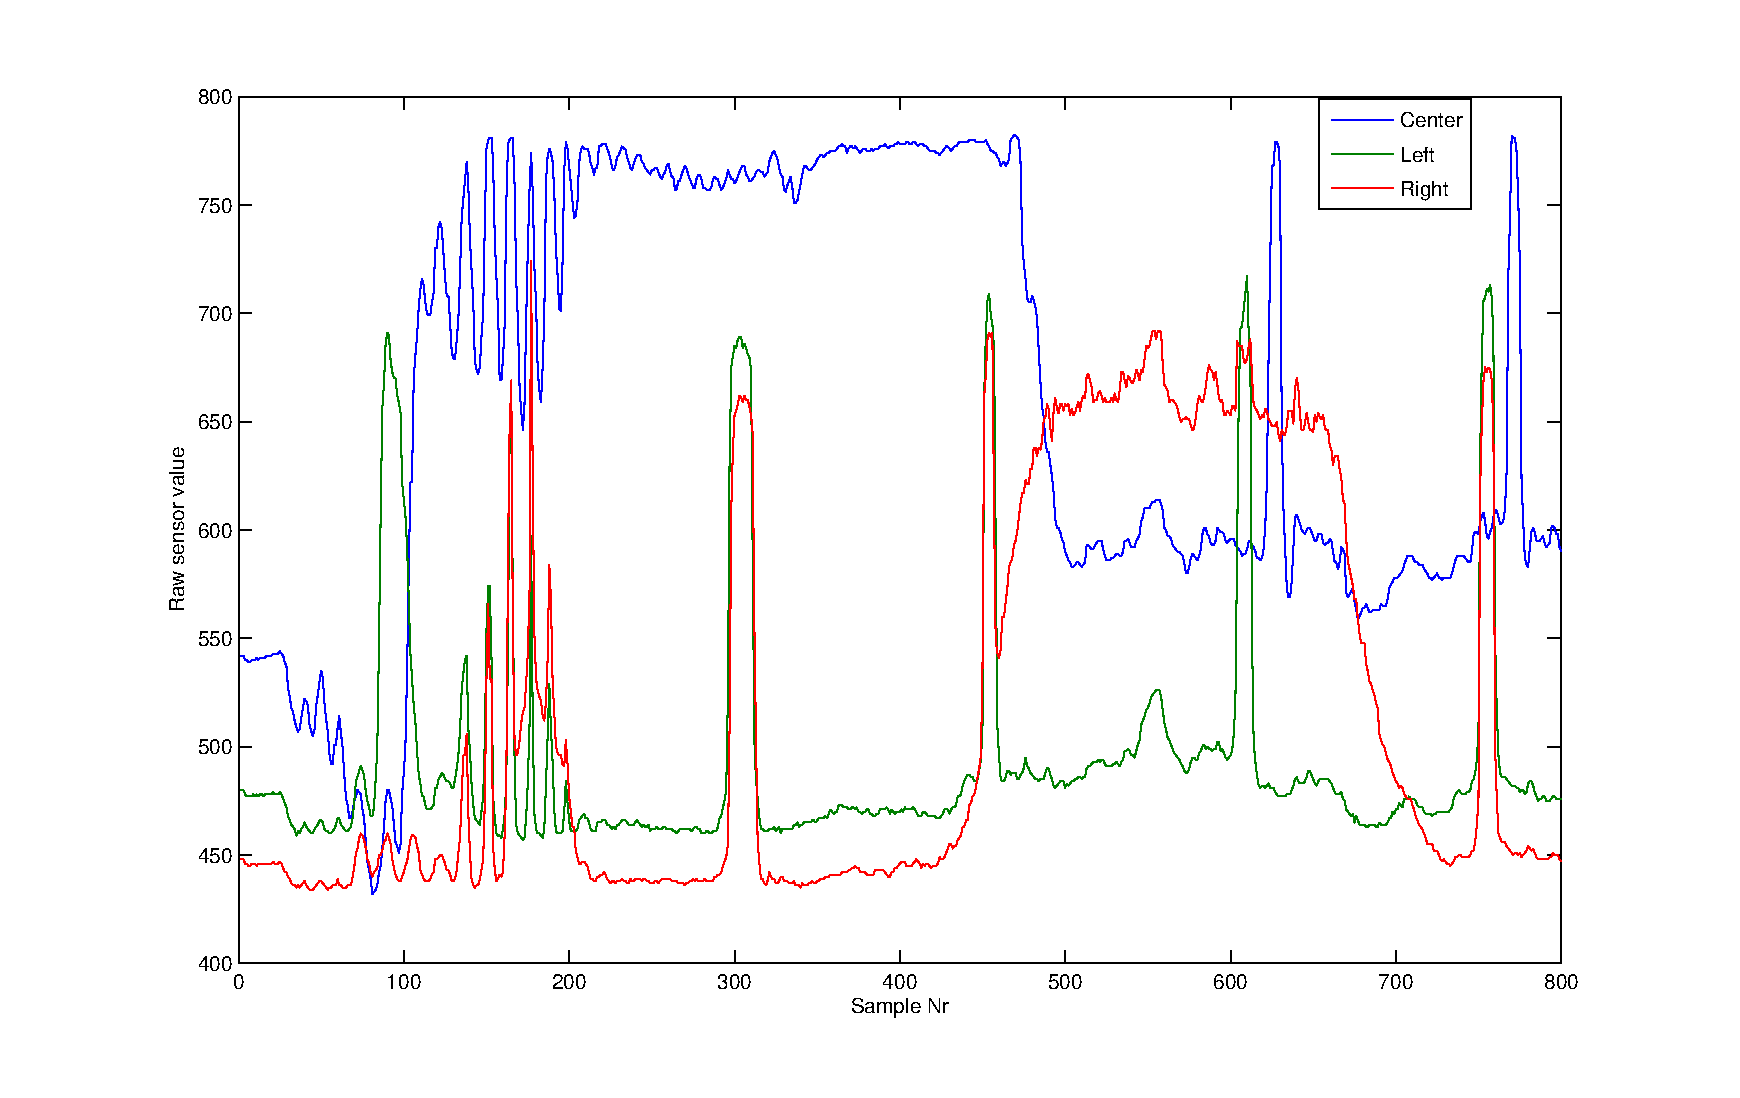
\includegraphics[scale=0.45]{sensor_measurements}
	            \caption{Raw samples of sensor measurements}\label{fig:sensor_measurements}
            \end{figure}
            \\
            \paragraph{Statemachine based}
            For making the control loop two different implementations has been
            tested, one using a simple state machine based solution, where the
            state machine tries to assess the position of the line as either left of the
            vehicle, centered below the vehicle or right of the vehicle and from
            this assessment tries to correct.\\
            \\
            \paragraph{PD-feedback based}
            Another option which has been tested is making a simple PD control loop
            using the light sensors, as the sensors are not entirely binary,
            but has a slight transition as more and more of the sensed area becomes
            line, it increases, a correction based on these small increases can 
            be seen as the oscillation between sample 100 - 200 on figure \ref{fig:sensor_measurements}
            Whereas the state machine based approach does not start correcting before reaching a threshold value.\\
            \\
            Having implemented both solutions on the vehicle the control loop based
            solution was chosen as it had the best performance.
		    %More detailed problem description with sensor position drawing
		    %measurement data examples.
		    %From there show proposed solutions
		    %Explain which one was chosen for which reasons, show flow diagrams
		    %of these two algorithms 
		    %Show incoming and output data from this block and the module test
%		    What is the responsibility of this block
%			Block interface
%			Block design / bird perspective flow chart 
%			Block test
	\subsection{Conclusion} %Morten
	    \fixme{Let us write this when the vehicle is done}
\section{Planner description}
    \subsection{Problem discussion, in the Sokoban domain}
Sokoban is a game originating from Japan. The essence of the game is to push jewels around in a room containing obstacles, in a manner that will enable the player to place all the jewels on so called goals in the room. See figure \ref{fig:sokohero} for a screenshot of a sokoban game.
Sokoban is an interesting game to study in the domain of Artificial Intelligence, because it presents a so called NP-complete problem, meaning in this case that it is often fairly easy for humans to solve such puzzles in a manner of minutes, but very difficult to develop an efficient algorithm able to do the same. This is due to the fact that NP-complete problems spawn huge search trees and branch factors.

\subsubsection{The rules of the game}
The rules of the game are simple. The game is best described as consisting of squares, each having an (x, y) coordinate. A game consists of the following squares:
\begin{itemize}
\item One 'Man' square, representing the player. The 'Man' square can move around.
\item One or more 'Jewel' squares representing objects that have to be pushed onto 'Goal' squares by the player.
\item One or more 'Goal' squares. There are always the same amount of 'goal' squares as 'Jewel' squares.
\item One or more 'Wall' representing impenetrable boundaries which can not be passed by neither 'Man' nor 'Jewel' squares.
\item One or more 'Empty' squares representing space where the player/'Man' square is able to move. 
\end{itemize}

\begin{figure}[ht]
\centering
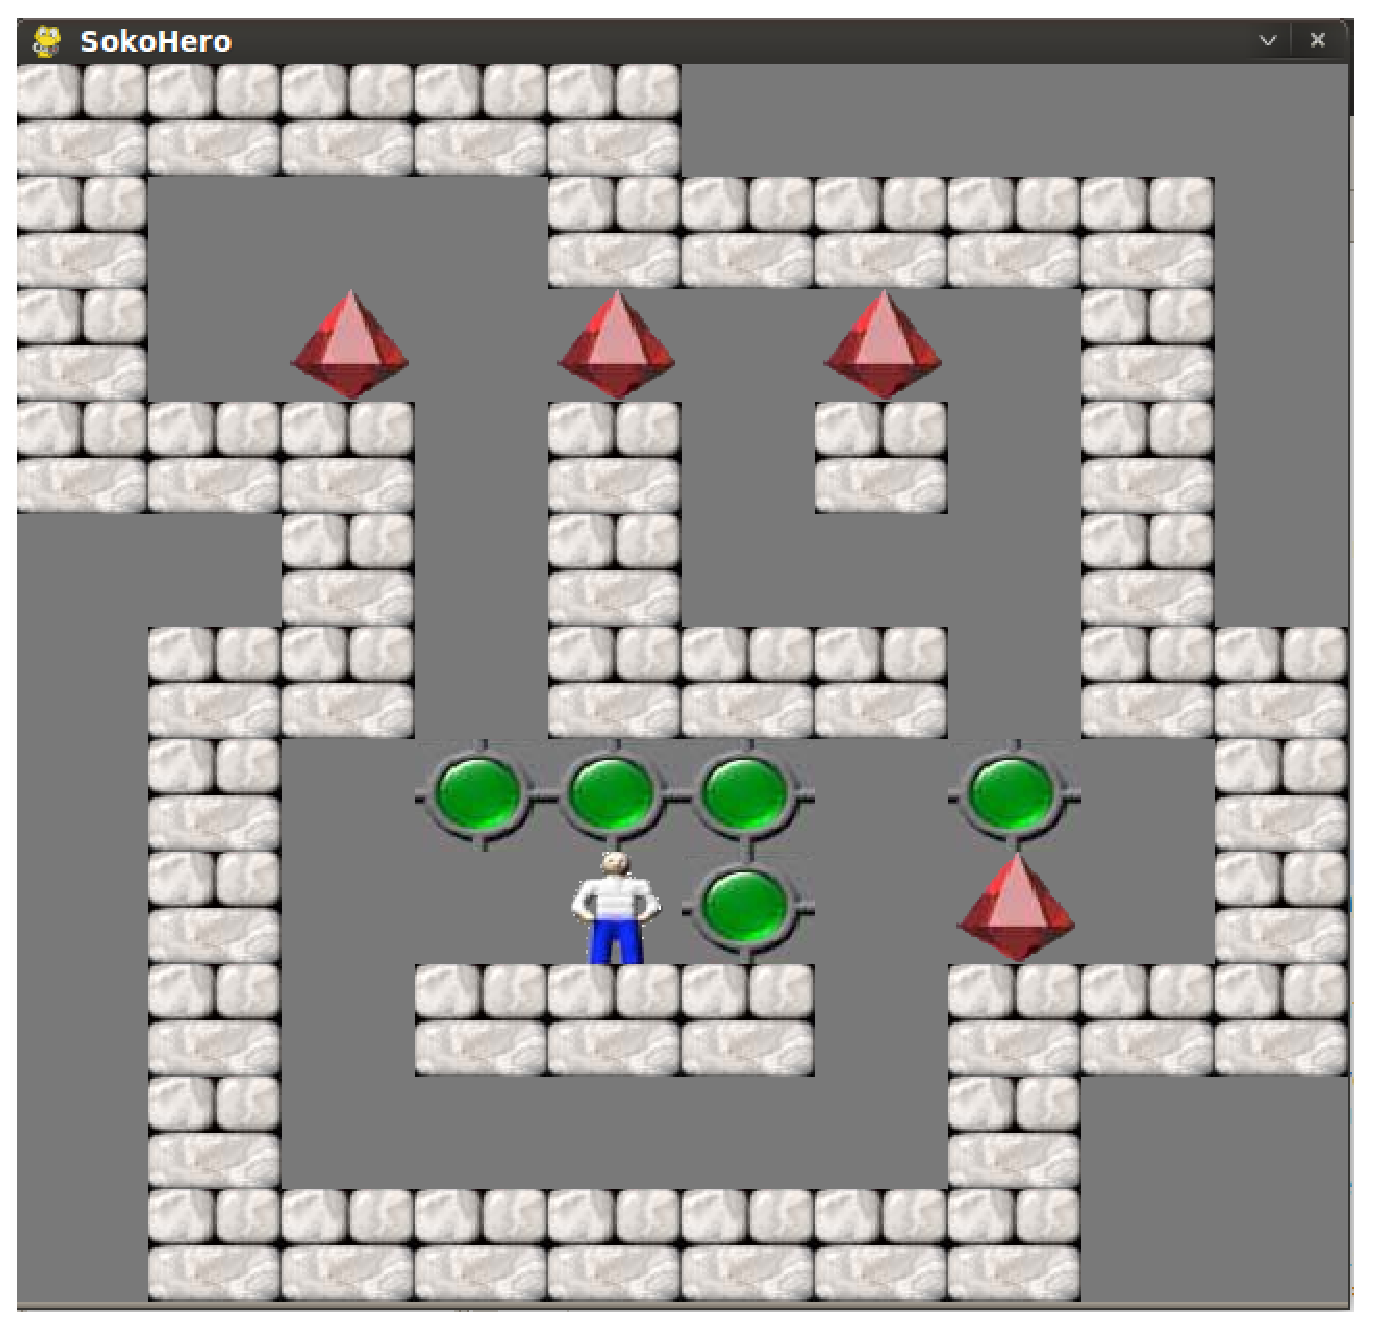
\includegraphics[scale=0.25]{images/sokohero.eps}
\caption{A screenshot of a sokoban game}
\label{fig:sokohero}
\end{figure}


As stated previously the purpose of the game is for the player to push 'Jewel' squares onto 'Goal' squares. That the player is only able to push jewels signifies that if a jewel is at position (x, y), and the player is at position (x - 1, y) then the player will be able to move the jewel to position (x + 1, y) if (x + 1, y) is occupied by an 'Empty' or a 'Goal' square. The same logic applies for other directions.
 
\subsubsection{Challenges faced when solving Sokoban algorithmically}
Given the fact that the player can on average move up, down, left and right, we see that the problem presents a so called branching factor of 4. If an algorithm is able to solve the puzzle in 100 moves, the complexity becomes 4$^{100}$ . 
This enormous complexity, illustrates the need for some sort of heuristics or pruning of the search tree, if the problem is to be solved in an acceptable time frame.
Deadlocks are one of the main challenges faced when trying to solve the Sokoban puzzle. A deadlock is best described as a situation where a jewel is pushed into a position that eliminates the possibility of solving the puzzle, for instance pushing a jewel into a corner. 

\subsubsection{Algorithmic approach}
The general approach taken to solve the sokoban problem, is creating a search tree where every node in the tree is a state of the game. The goal is then to traverse the tree to find the state where all of the coordinates of the jewels match the coordinates of all the goals.\\
The general algorithmic search can described as:

\begin{lstlisting}[language=Ruby, frame=single, basicstyle=\tiny, caption={Deadlock detection pseudo code}, label={code:sokoalgo}]
if not problem solved:
	get next state in search tree
	if state not goal state:
	  for each jewel in state do:
	    for every direction in which jewel can move one square do:
		  if resulting state is valid and not duplicate of a previous state:
		   if robot can get to the position to push the jewel in the desired direction:
             create new state				
			 move jewel to new position
			 move robot to previous jewel position
			 calculate state score
			 add state to search tree	
\end{lstlisting}

As can be seen from the pseudo code, the problem solving can logically be divided into two separate subproblems, the first one being the movement of the jewels, henceforth known as the jewel problem, and the second being the path finding from the robot to the jewel that has to be moved, henceforth known as the path finding problem. 
The search approach best suited for the solving of these two distinct areas might not be the same, and therefore each subproblem is considered separately, and the solution implemented will treat the subproblems as two seperate search trees. 
It is important to note that the optimal solutions is wanted in terms of minimum number of robot/man movements. This is as mentioned due to the fact that the competition is on time, and the assumption therefore is that the less squares that the robot has to traverse, the less time it will take to solve the puzzle.
	\subsection{Discussion of path finding algorithms} %Mikael
		\subsubsection{Selection of algorithm}
		1\section{Map representation}
The particular Sokoban puzzle that must be solved by the robot, is handed out beforehand in a textual format. An example of this textual format is:
\\\\
XXXXX\\  
X......XXXXX\\ 
X..J..J..J...X\\  
XXX..X..X...X\\   
\hspace*{6 mm}X..X.....X\\  
\hspace*{3 mm}XX..XXX..XX\\        
\hspace*{3 mm}X..GGG..G..X\\ 
\hspace*{3 mm}X....MG..J..X\\  
\hspace*{3 mm}X..XXX..XXX\\     
\hspace*{3 mm}X............X\\
\hspace*{3 mm}XXXXXXX  
\\\\ 
where 'X' represents 'Wall' squares, '.' represent 'Emtpy' squares, 'J' represents 'Jewel' squares, 'G' represents 'goal' squares and finally 'M' represents the 'Man' square. 

This map representation will be converted directly into a multidimensional array, in order to use the map in graph traversal by the chosen search algorithm. The multidimensional array representation is preferable, because a particular squares x and y coordinate translates directly to the corresponding row and column of the multidimensional array, which in turn enables the algorithm to quickly look up possible routes. %Mikael
	\subsection{Algorithm design}
	\subsection{Performance evaluation}
	\subsection{conclusion}
\section{Conclusion}
\section{Discussion}
\bibliographystyle{plain}
\bibliography{bibtex_refs.bib}
\appendix
\end{document}

